\documentclass[twoside]{book}

% Packages required by doxygen
\usepackage{fixltx2e}
\usepackage{calc}
\usepackage{doxygen}
\usepackage[export]{adjustbox} % also loads graphicx
\usepackage{graphicx}
\usepackage[utf8]{inputenc}
\usepackage{makeidx}
\usepackage{multicol}
\usepackage{multirow}
\PassOptionsToPackage{warn}{textcomp}
\usepackage{textcomp}
\usepackage[nointegrals]{wasysym}
\usepackage[table]{xcolor}

% Font selection
\usepackage[T1]{fontenc}
\usepackage[scaled=.90]{helvet}
\usepackage{courier}
\usepackage{amssymb}
\usepackage{sectsty}
\renewcommand{\familydefault}{\sfdefault}
\allsectionsfont{%
  \fontseries{bc}\selectfont%
  \color{darkgray}%
}
\renewcommand{\DoxyLabelFont}{%
  \fontseries{bc}\selectfont%
  \color{darkgray}%
}
\newcommand{\+}{\discretionary{\mbox{\scriptsize$\hookleftarrow$}}{}{}}

% Page & text layout
\usepackage{geometry}
\geometry{%
  a4paper,%
  top=2.5cm,%
  bottom=2.5cm,%
  left=2.5cm,%
  right=2.5cm%
}
\tolerance=750
\hfuzz=15pt
\hbadness=750
\setlength{\emergencystretch}{15pt}
\setlength{\parindent}{0cm}
\setlength{\parskip}{3ex plus 2ex minus 2ex}
\makeatletter
\renewcommand{\paragraph}{%
  \@startsection{paragraph}{4}{0ex}{-1.0ex}{1.0ex}{%
    \normalfont\normalsize\bfseries\SS@parafont%
  }%
}
\renewcommand{\subparagraph}{%
  \@startsection{subparagraph}{5}{0ex}{-1.0ex}{1.0ex}{%
    \normalfont\normalsize\bfseries\SS@subparafont%
  }%
}
\makeatother

% Headers & footers
\usepackage{fancyhdr}
\pagestyle{fancyplain}
\fancyhead[LE]{\fancyplain{}{\bfseries\thepage}}
\fancyhead[CE]{\fancyplain{}{}}
\fancyhead[RE]{\fancyplain{}{\bfseries\leftmark}}
\fancyhead[LO]{\fancyplain{}{\bfseries\rightmark}}
\fancyhead[CO]{\fancyplain{}{}}
\fancyhead[RO]{\fancyplain{}{\bfseries\thepage}}
\fancyfoot[LE]{\fancyplain{}{}}
\fancyfoot[CE]{\fancyplain{}{}}
\fancyfoot[RE]{\fancyplain{}{\bfseries\scriptsize Generated by Doxygen }}
\fancyfoot[LO]{\fancyplain{}{\bfseries\scriptsize Generated by Doxygen }}
\fancyfoot[CO]{\fancyplain{}{}}
\fancyfoot[RO]{\fancyplain{}{}}
\renewcommand{\footrulewidth}{0.4pt}
\renewcommand{\chaptermark}[1]{%
  \markboth{#1}{}%
}
\renewcommand{\sectionmark}[1]{%
  \markright{\thesection\ #1}%
}

% Indices & bibliography
\usepackage{natbib}
\usepackage[titles]{tocloft}
\setcounter{tocdepth}{3}
\setcounter{secnumdepth}{5}
\makeindex

% Hyperlinks (required, but should be loaded last)
\usepackage{ifpdf}
\ifpdf
  \usepackage[pdftex,pagebackref=true]{hyperref}
\else
  \usepackage[ps2pdf,pagebackref=true]{hyperref}
\fi
\hypersetup{%
  colorlinks=true,%
  linkcolor=blue,%
  citecolor=blue,%
  unicode%
}

% Custom commands
\newcommand{\clearemptydoublepage}{%
  \newpage{\pagestyle{empty}\cleardoublepage}%
}

\usepackage{caption}
\captionsetup{labelsep=space,justification=centering,font={bf},singlelinecheck=off,skip=4pt,position=top}

%===== C O N T E N T S =====

\begin{document}

% Titlepage & ToC
\hypersetup{pageanchor=false,
             bookmarksnumbered=true,
             pdfencoding=unicode
            }
\pagenumbering{alph}
\begin{titlepage}
\vspace*{7cm}
\begin{center}%
{\Large My Project }\\
\vspace*{1cm}
{\large Generated by Doxygen 1.8.13}\\
\end{center}
\end{titlepage}
\clearemptydoublepage
\pagenumbering{roman}
\tableofcontents
\clearemptydoublepage
\pagenumbering{arabic}
\hypersetup{pageanchor=true}

%--- Begin generated contents ---
\chapter{File Index}
\section{File List}
Here is a list of all documented files with brief descriptions\+:\begin{DoxyCompactList}
\item\contentsline{section}{\hyperlink{buffer_8c}{buffer.\+c} \\*Struct and function for buffer management }{\pageref{buffer_8c}}{}
\item\contentsline{section}{\hyperlink{buffer_8h}{buffer.\+h} \\*Header file for buffer management }{\pageref{buffer_8h}}{}
\item\contentsline{section}{\hyperlink{calculator_8c}{calculator.\+c} \\*Calculator implementation }{\pageref{calculator_8c}}{}
\item\contentsline{section}{\hyperlink{calculator_8h}{calculator.\+h} \\*Header file for Calculator }{\pageref{calculator_8h}}{}
\item\contentsline{section}{\hyperlink{convert_8c}{convert.\+c} \\*Infix-\/to-\/postfix convertor }{\pageref{convert_8c}}{}
\item\contentsline{section}{\hyperlink{convert_8h}{convert.\+h} \\*Header file for infix to postfix convertor }{\pageref{convert_8h}}{}
\item\contentsline{section}{\hyperlink{main_8c}{main.\+c} \\*Calculator program reads the string of numeric infix expression, converts it postfix expression, calculates the postfix expression and prints out the result }{\pageref{main_8c}}{}
\item\contentsline{section}{\hyperlink{stack_8c}{stack.\+c} \\*Stack implementation for symbols }{\pageref{stack_8c}}{}
\item\contentsline{section}{\hyperlink{stack_8h}{stack.\+h} \\*Header file for stack implementation }{\pageref{stack_8h}}{}
\item\contentsline{section}{\hyperlink{utility_8h}{utility.\+h} \\*Utility macros }{\pageref{utility_8h}}{}
\end{DoxyCompactList}

\chapter{File Documentation}
\hypertarget{my__mod_8c}{}\section{my\+\_\+mod.\+c File Reference}
\label{my__mod_8c}\index{my\+\_\+mod.\+c@{my\+\_\+mod.\+c}}


Test codes to study kernel module.  


{\ttfamily \#include $<$linux/init.\+h$>$}\newline
{\ttfamily \#include $<$linux/module.\+h$>$}\newline
{\ttfamily \#include $<$linux/kernel.\+h$>$}\newline
Include dependency graph for my\+\_\+mod.\+c\+:
\nopagebreak
\begin{figure}[H]
\begin{center}
\leavevmode
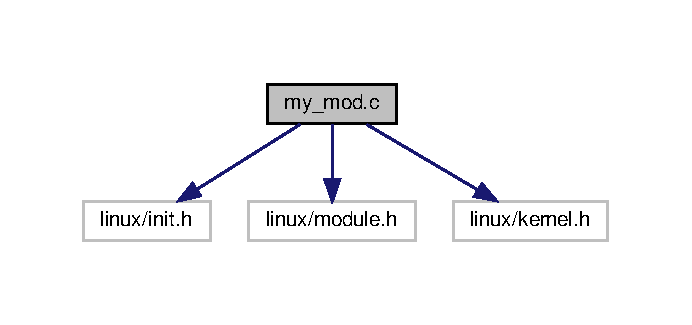
\includegraphics[width=332pt]{my__mod_8c__incl}
\end{center}
\end{figure}
\subsection*{Functions}
\begin{DoxyCompactItemize}
\item 
\mbox{\Hypertarget{my__mod_8c_aaee9b4944367015e0fc61caadc10c0ca}\label{my__mod_8c_aaee9b4944367015e0fc61caadc10c0ca}} 
\hyperlink{my__mod_8c_aaee9b4944367015e0fc61caadc10c0ca}{module\+\_\+init} (my\+\_\+mod\+\_\+init)
\begin{DoxyCompactList}\small\item\em Macro declaration to expose init function of this module. \end{DoxyCompactList}\item 
\mbox{\Hypertarget{my__mod_8c_ae872d5bbea4c8f812e608e8dc7db6074}\label{my__mod_8c_ae872d5bbea4c8f812e608e8dc7db6074}} 
\hyperlink{my__mod_8c_ae872d5bbea4c8f812e608e8dc7db6074}{module\+\_\+exit} (my\+\_\+mod\+\_\+exit)
\begin{DoxyCompactList}\small\item\em Macro declaration to expose exit function of this module. \end{DoxyCompactList}\item 
\mbox{\Hypertarget{my__mod_8c_ad94b36675e7eb067ea3ce6ff9e244a44}\label{my__mod_8c_ad94b36675e7eb067ea3ce6ff9e244a44}} 
\hyperlink{my__mod_8c_ad94b36675e7eb067ea3ce6ff9e244a44}{M\+O\+D\+U\+L\+E\+\_\+\+L\+I\+C\+E\+N\+SE} (\char`\"{}G\+PL\char`\"{})
\begin{DoxyCompactList}\small\item\em Macro for license of this module. \end{DoxyCompactList}\item 
\mbox{\Hypertarget{my__mod_8c_ad4ab8285f8a6d5c3455f8285348695f7}\label{my__mod_8c_ad4ab8285f8a6d5c3455f8285348695f7}} 
\hyperlink{my__mod_8c_ad4ab8285f8a6d5c3455f8285348695f7}{M\+O\+D\+U\+L\+E\+\_\+\+A\+U\+T\+H\+OR} (\char`\"{}Youngeun Park\char`\"{})
\begin{DoxyCompactList}\small\item\em Macro for the author of this module. \end{DoxyCompactList}\item 
\mbox{\Hypertarget{my__mod_8c_a79015fa990f0d83ee6cf43f4a2440c53}\label{my__mod_8c_a79015fa990f0d83ee6cf43f4a2440c53}} 
\hyperlink{my__mod_8c_a79015fa990f0d83ee6cf43f4a2440c53}{M\+O\+D\+U\+L\+E\+\_\+\+D\+E\+S\+C\+R\+I\+P\+T\+I\+ON} (\char`\"{}Test module to learn Kernel module A\+PI\char`\"{})
\begin{DoxyCompactList}\small\item\em Macro for the description of this module. \end{DoxyCompactList}\end{DoxyCompactItemize}


\subsection{Detailed Description}
Test codes to study kernel module. 

\begin{DoxyDate}{Date}
2018/06/27 
\end{DoxyDate}
\begin{DoxyAuthor}{Author}
Youngeun Park 
\end{DoxyAuthor}

%--- End generated contents ---

% Index
\backmatter
\newpage
\phantomsection
\clearemptydoublepage
\addcontentsline{toc}{chapter}{Index}
\printindex

\end{document}
